%----------------------------------------------------------------------------------------
% METADATA BLOCK (YAML)  — see inbox/README.md for every field
%----------------------------------------------------------------------------------------
% uid: ""
% school: "lycee"
% level: "3eme"
% section: "Mathématiques"
% chapter: "Rotations"
% title: "Bonus : le théorème de Pompeiu"
% difficulty: "Moyen"
% tags: ["pompeiu", "rotation", "triangle-equilateral", "nombres-complexes", "cercle-circonscrit"]
% provenance: "adapted"
% batch: "2026-11-20-defis-geometrie-A"
% defi: true
%----------------------------------------------------------------------------------------

\newcommand{\R}{\mathbb{R}}

% ---STATEMENT---
Soit $ABC$ un triangle équilatéral et $P$ un point quelconque du plan. On veut montrer que \textbf{$PA$, $PB$, $PC$ sont les longueurs des côtés d'un triangle, et que ce triangle est aplati si et seulement si $P$ est sur le cercle circonscrit à $ABC$.}

% alt: Triangle équilatéral ABC, son cercle circonscrit en pointillés et un point P quelconque
\begin{center}
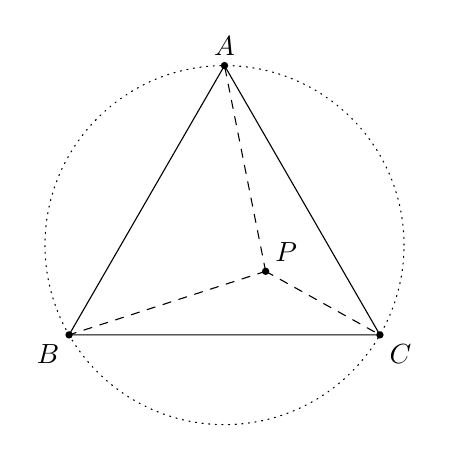
\begin{tikzpicture}[scale=0.95,line cap=round,line join=round,>=stealth]
\draw[dotted] (0,0) circle (2.4);
\draw (0,2.4) -- (-2.078,-1.2) -- (2.078,-1.2) -- cycle;
\draw[dashed] (0.55,-0.35) -- (0,2.4);
\draw[dashed] (0.55,-0.35) -- (-2.078,-1.2);
\draw[dashed] (0.55,-0.35) -- (2.078,-1.2);
\fill(0,2.4) circle (1.4pt) node[above] {$A$};
\fill(-2.078,-1.2) circle (1.4pt) node[below left] {$B$};
\fill(2.078,-1.2) circle (1.4pt) node[below right] {$C$};
\fill(0.55,-0.35) circle (1.4pt) node[above right] {$P$};
\end{tikzpicture}
\end{center}

\begin{enumerate}
  \item On suppose $ABC$ direct. Soit $\rho$ la rotation de centre $B$ qui envoie $A$ sur $C$ et $P'=\rho(P)$.
  \begin{enumerate}
    \item Montrer que le triangle $BPP'$ est équilatéral et que $P'C=PA$.
    \item En déduire que $PA\leq PB+PC$, $PB\leq PC+PA$ et $PC\leq PA+PB$ : les trois nombres sont les longueurs des côtés d'un triangle (éventuellement aplati).
  \end{enumerate}
  \item On munit le plan d'un repère orthonormé direct d'origine le centre de $ABC$, tel que $A$, $B$, $C$ aient pour affixes $1$, $j$, $j^2$, où $j=e^{2i\pi/3}$. Soit $p$ l'affixe de $P$.
  \begin{enumerate}
    \item Montrer que $(p-1)+j(p-j)+j^2(p-j^2)=0$.
    \item En déduire que le triangle de côtés $PA$, $PB$, $PC$ est aplati si et seulement si les nombres $p-1$, $j(p-j)$, $j^2(p-j^2)$ sont « alignés » (leurs images sont sur une même droite passant par $O$).
    \item Montrer que $\mathrm{Im}\left[\bar j\,(p-1)\,\overline{(p-j)}\right]=\dfrac{\sqrt3}{2}\left(1-|p|^2\right)$, puis que le triangle est aplati si et seulement si $|p|=1$.
  \end{enumerate}
\end{enumerate}

% ---SOLUTION---
\begin{enumerate}[itemsep=14pt]
  \item\leavevmode
  \begin{enumerate}[itemsep=8pt]
    \item\leavevmode
    \begin{prop}[Rotation]
    Une rotation conserve les distances. Si une rotation de centre $B$ envoie $P$ sur $P'$ , alors $BP'=BP$ et $\widehat{PBP'}$ est égal à l'amplitude de la rotation.
    \end{prop}
    $\rho$ envoie $A$ sur $C$ avec $BA=BC$ et $\widehat{ABC}=60^\circ$ : c'est une rotation d'amplitude $60^\circ$.

    Donc $BP'=BP$ et $\widehat{PBP'}=60^\circ$ : le triangle $BPP'$ est isocèle avec un angle de $60^\circ$ en $B$, donc équilatéral, et $PP'=PB$.

    $\rho(A)=C$ et $\rho(P)=P'$ ; une rotation conserve les distances : $CP'=AP$.
    \item Dans le triangle $PCP'$ (éventuellement aplati), les côtés sont
    \[PC,\qquad CP'=PA,\qquad PP'=PB.\]
    \begin{prop}[Inégalité triangulaire]
    Pour trois points $U,V,W$ : \ib{$UV\leq UW+WV$}, avec égalité si et seulement si $W\in[UV]$.
    \end{prop}
    Donc $PP'\leq PC+CP'$, soit $PB\leq PC+PA$ ; et $PC\leq PP'+P'C=PB+PA$ ; et $CP'\leq CP+PP'$, soit $PA\leq PC+PB$.
  \end{enumerate}

  \item\leavevmode
  \begin{enumerate}[itemsep=8pt]
    \item $p(1+j+j^2)-(1+j\cdot j+j^2\cdot j^2)=p\times0-(1+j^2+j^4)$.

    Comme $j^3=1$ : $j^4=j$, et $1+j+j^2=0$. Donc $1+j^2+j=0$ et la somme est nulle.
    \item Posons $x=p-1$, $y=j(p-j)$, $z=j^2(p-j^2)$ : $|x|=PA$, $|y|=PB$, $|z|=PC$ (car $|j|=1$) et $x+y+z=0$.

    Les trois nombres forment un triangle fermé de côtés $PA,PB,PC$ (on place $y$ puis $z$ bout à bout à partir de $x$). Ce triangle est aplati si et seulement si $x,y,z$ sont parallèles (sur une même droite), c'est-à-dire :
    \[x\bar y\in\R\quad(\text{si }x,y\neq0).\]
    \item $x\bar y=(p-1)\,\bar j\,\overline{(p-j)}$. On développe :
    \[(p-1)\overline{(p-j)}=|p|^2-\bar j\,p-\bar p+\bar j.\]
    On multiplie par $\bar j$ (avec $\bar j^2=j$) : $\ \bar j|p|^2-j\,p-\bar j\,\bar p+j$.

    Le nombre $j\,p+\bar j\,\bar p=2\,\mathrm{Re}(jp)$ est réel : il n'a pas de partie imaginaire. Reste
    \[\mathrm{Im}\left(\bar j\,|p|^2+j\right)=-\dfrac{\sqrt3}{2}|p|^2+\dfrac{\sqrt3}{2}=\ib{$\dfrac{\sqrt3}{2}\left(1-|p|^2\right)$}.\]
    Donc $x\bar y\in\R\iff|p|^2=1\iff|p|=1$.

    \emph{Conclusion.} Si $P$ est sur le cercle circonscrit ($|p|=1$), $x\parallel y$ ; et $z=-x-y$ est parallèle aussi : le triangle est aplati. Si $|p|\neq1$, $x\bar y\notin\R$, donc $x$ et $y$ ne sont pas parallèles (ils sont non nuls car $P\neq A,B$ quand $|p|\neq1$) : le triangle n'est pas aplati. $\blacksquare$
  \end{enumerate}
\end{enumerate}

\textbf{Remarque.} Dans le cas aplati, l'une des trois longueurs est la somme des deux autres : c'est le théorème de Ptolémée appliqué au quadrilatère $ABPC$ ou à l'un de ses analogues.

\textbf{Idée :} une seule rotation de $60^\circ$ rassemble $PA$, $PB$, $PC$ en un triangle $PCP'$ ; la version complexe est la même idée : $1+j+j^2=0$ ferme le triangle de côtés $p-1$, $j(p-j)$, $j^2(p-j^2)$.

\textbf{Piège :} quand $P$ est un sommet (par exemple $P=A$), la longueur $PA=0$ ; le « triangle » a un côté nul, mais reste un cas d'aplatissement ($|p|=1$).
